\section{$\ee \rightarrow \ttbar$ at threshold}
One of the unique capabilities of an $\ee$ linear collider is the ability
to carry out cross section measurements at particle 
production thresholds.  The accurately known and readily variable beam 
energy of the ILC makes it possible to measure the shape of the cross section
at any pair-production threshold within its range.
Because of the leptonic initial state, it is also  possible to tune 
the initial spin state, giving additional options for precision threshold 
measurements. 
The $t\bar t$ pair production threshold, located at a center of mass energy
energy  $\sqrt{s}\approx 2 m_t$,  allows for precise measurements of 
the $t$~quark mass $m_t$ as well as the $t$~quark 
total width $\Gamma_t$ and the QCD coupling $\alpha_s$. 
 Because the top is a spin-$\frac{1}{2}$ fermion, the
 $t\bar t$ pair is produced in an angular $S$-wave state.  This leads to
a clearly visible rise of the cross section even when folded with the
 ILC luminosity spectrum. Moreover, because the top pair is 
produced in a color singlet state, the experimental measurements can be 
compared with very accurate and unambiguous 
analytic theoretical predictions of the cross section 
with negligible hadronization effects. The dependence of the 
$t$~quark cross section shape on the $t$~quark mass and interactions
is computable to high precision with full control over the renormalization 
scheme dependence of the top mass parameter.  In this section, we will 
review the expectations for the theory and ILC measurements of the 
$t$~quark threshold cross section shape. The case of the $t$~quark
threshold is not only important in its own right but also serves
 as a prototype case for other particle thresholds that might be accessible at the ILC.

\subsection{ Status of QCD theory}

The calculation of the total top pair production cross section makes use of the 
 method of non-relativistic effective 
theories. The $t$~quark mass parameter used in this calculation is
defined at the scale of about 10~GeV corresponding to the typical physical
separation of the $t$ and $\bar t$.  This mass parameter can be
converted to the $\msb$ mass in a controlled way. The summation of QCD
 Coulomb singularities treated by a 
non-relativistic fixed-order expansion is well known up to 
NNLO~\cite{Hoang:2000yr} and has recently been extended accounting 
also for NNNLO corrections~\cite{Beneke:2008cr}. Large QCD velocity 
logarithms have been determined using renormalization-group-improved 
non-relativistic perturbation theory up to NLL order, with a partial 
treatment of NNLL effects~\cite{Hoang:2001mm,Hoang:2003ns,Pineda:2006ri}.
Recently the dominant ultrasoft NNLL corrections have been 
completed~\cite{Hoang:2006ht,Pineda:2011aw,Hoang:2011gy}. The accuracy
in this calculation is illustrated in Fig.~\ref{fig:tthresh-hs}.

%%%%%%%%%%%%%%%%%%%%%%%%%%%%
\begin{figure}
\centering
%\includegraphics[width=0.7\columnwidth]{ttthresh_hs.pdf}
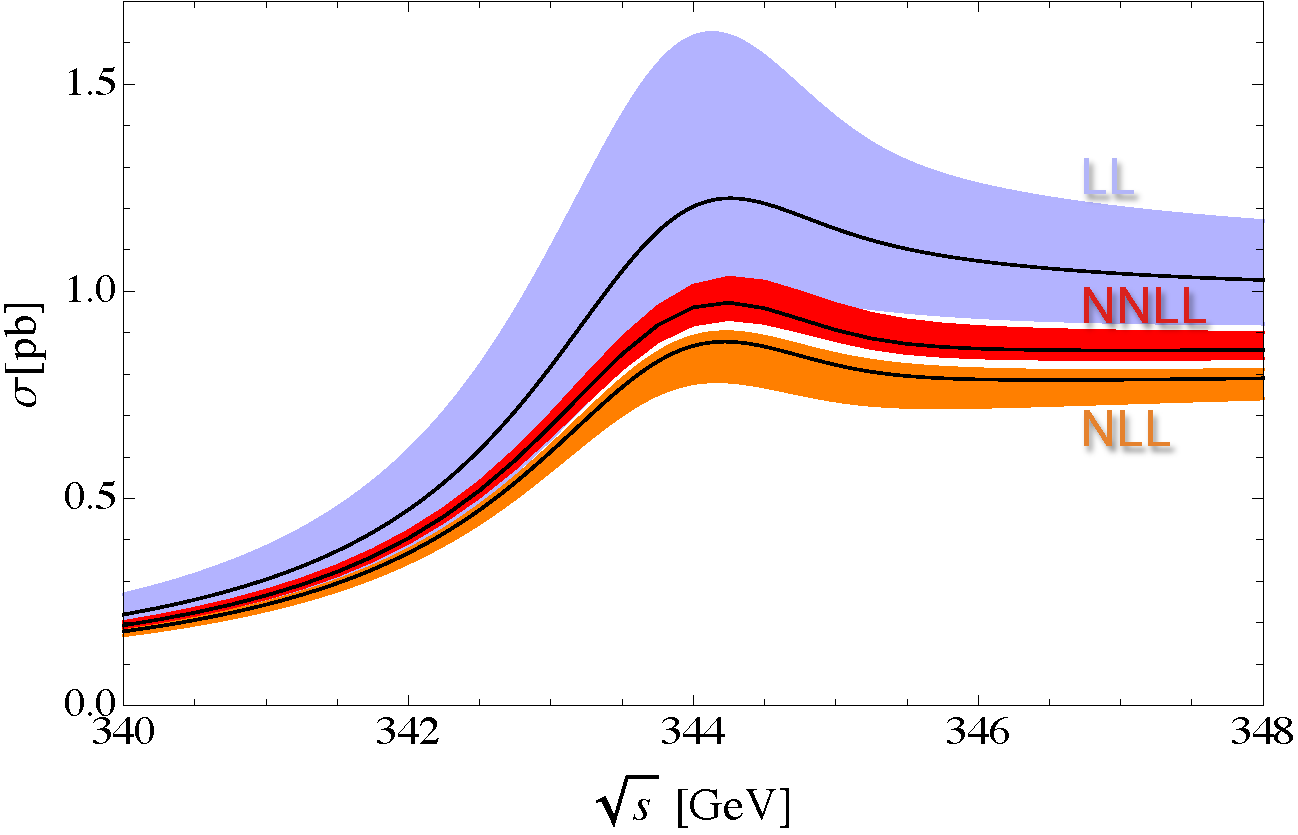
\includegraphics[width=0.7\columnwidth]{TotCrossCombined.pdf}
\caption{
%Accuracy on the prediction of the top pair production 
%cross section at the $t\bar{t}$~threshold at the ILC as achieved by 
%recent calculations of QCD corrections (NNLL). For further explanations 
%see text. The figure has been taken from~\cite{bib:topws-ms}.
Bands show the theoretical QCD uncertainties of the prediction of the top pair production cross section at the $t\bar t$ threshold
   at the ILC as achieved by recent renormalization-group-improved QCD calculations~\cite{Hoang:2013uda}. Their analysis estimated 
   the theoretical uncertainty in the total cross section as $d\sigma_{t\bar t}/\sigma_{t\bar t}\pm 5\%$. For further explanation see text.
}
\label{fig:tthresh-hs}
\end{figure}
%%%%%%%%%%%%%%%%%%%%%%%%%%%%%%%


Since the $t$~quark kinetic energy is of the order of the $t$~quark width, 
electro-weak effects, which also include finite-lifetime and interference 
contributions, are crucial as well. This makes the cross section dependent 
on the experimental prescription concerning the reconstructed final state. 
%Results published in ~\cite{Beneke:2010mp,Hoang:2010gu,Penin:2011gg} put approximate NNLL order 
%predictions within reach. Recently the NLO resonant calculation of $\ttbar$ in the publications cited before has been extended to NNLO  accuracy~\cite{Jantzen:2013gpa}.
Recently the NLO non-resonant calculation of $\ttbar$ production in~\cite{Beneke:2010mp,Penin:2011gg} has been extended to NNLO accuracy~\cite{Hoang:2010gu,Jantzen:2013gpa}.

Theoretical predictions for differential cross sections such as the 
top momentum distribution and forward-backward 
asymmetries are only known at the NNLO level 
and are thus much less developed.

%%%%%%%%%%%%%%%%%%%%%%%%%%%%%%%%%%%%%%%%%%%%%%%%%%%%%
\begin{figure}
\centering
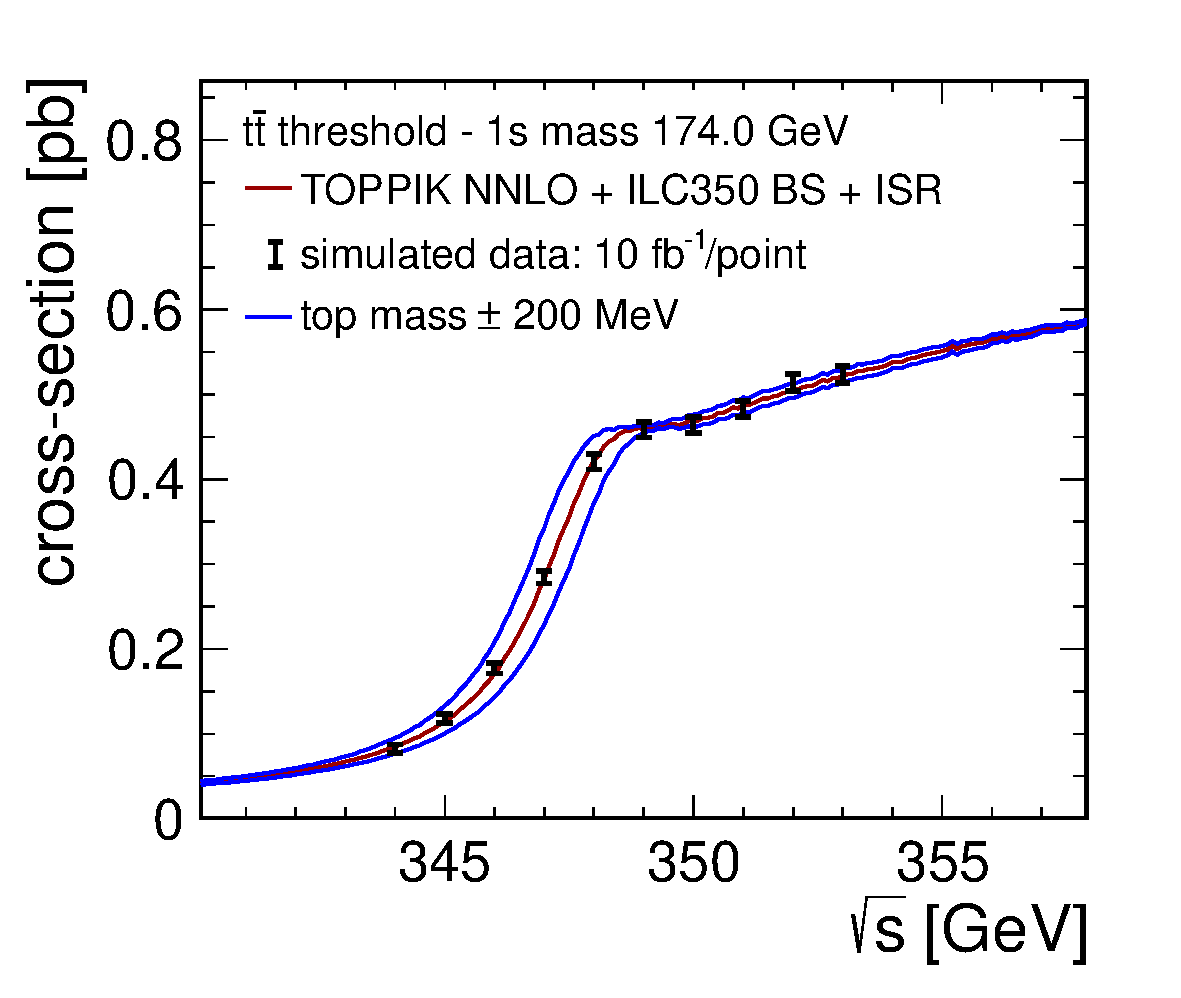
\includegraphics[width=0.50\columnwidth]{ILC_TopThreshold.pdf}
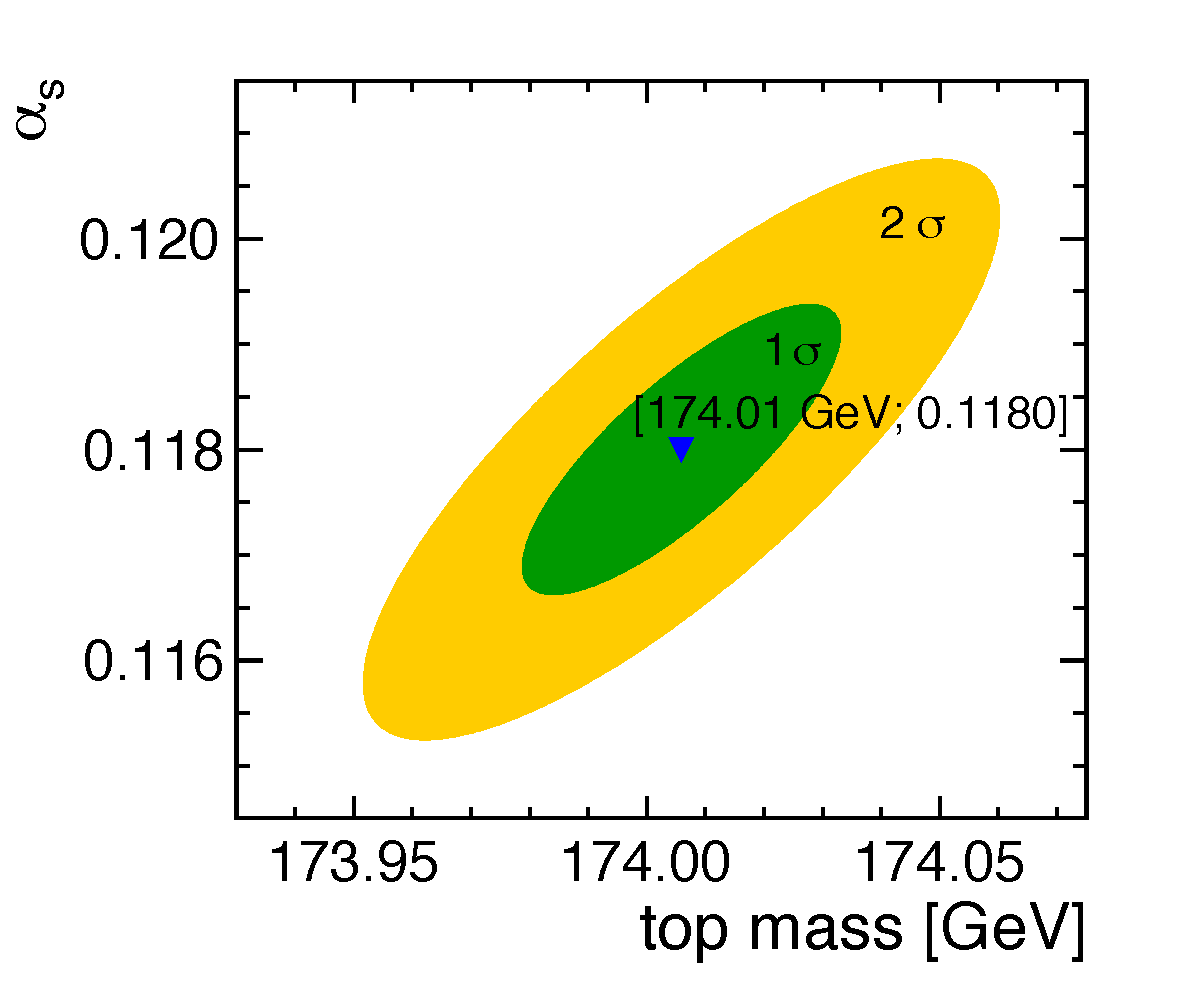
\includegraphics[width=0.40\columnwidth]{contours-10-ilc.pdf}
\caption{Illustration of a $t$~quark threshold measurement at the ILC. 
In the simulation, the $t$~quark mass has been 
chosen to be 174.~GeV.  The blue lines show the effect of varying this 
mass by 200~MeV. The study is based on full detector simulation and takes 
initial state radiation (ISR) and beamstrahlung (BS) and other relevant 
machine effects into account: (left) the simulated threshold scan.  (right) 
error ellipse for the determination of $m_t$ and $\alpha_s$. The figure is
 taken from~\cite{Seidel:2013sqa}.}
\label{fig:ttthresh-scan}
\end{figure}
%%%%%%%%%%%%%%%%%%%%%%%%%%%%%%%%%%%%%%%%%%%%%%%%%%%%%%%%%%%%%%%%
 
\subsubsection{Simulations and measurements}

The most recent experimental study has been carried out by Seidel, Simon, and Tesar, for which the 
results are shown in Fig.~\ref{fig:ttthresh-scan}~\cite{Seidel:2013sqa}. That study is based on a full detector simulation 
using the ILD detector. It takes the initial state radiation and beamstrahlung of the colliding beams into 
account. has been carried out by Martinez and Miquel in~\cite{Martinez:2002st}.
These authors assumed a total integrated luminosity of $100$~fb$^{-1}$, distributed over 10 equidistant energy points 
in a $10$~GeV range around the threshold, using the ILC and CLIC beam parameters. To treat the 
strong correlation of the input theory parameters, simultaneous fits 
were carried out for the $t$~quark mass, the QCD coupling and the $t$~quark width from 
measurements of the total cross section that was simulated based on the code TOPPIK with NNLO corrections~\cite{Hoang:1999zc}. 
The results are shown in Table~\ref{tab:ThresholdResults} and demonstrate that the statistical precision of the $t$~quark mass in this study is of the order of 30\,MeV.
The results are compatible with the results reported in~\cite{Horiguchi:2013wra}. There the width of the $t$ quark is determined to a statistical precision at the 2\% level.   

\begin{table}
\centering
\begin{tabular}{|ccc|}
\hline
\multicolumn{3}{|c|}{1S top mass and $\alpha_s$ combined 2D fit}\\
\hline
Error type & ILC & CLIC \\
\hline
 $m_t$ stat. error &  27~MeV & 34~MeV\\
 $m_t$ theory syst. (1\%/3\%) &  5~MeV / 9~MeV & 5~MeV / 8~MeV\\
 $\alpha_s$ stat. error & 0.0008 & 0.0009\\
 $\alpha_s$ theory syst. (1\%/3\%) & 0.0007 / 0.0022 & 0.0008 / 0.0022 \\
\hline
\end{tabular}

\caption{Results summary for the 2D simultaneous top mass and $\alpha_s$ determination with a threshold scan at CLIC and ILC for 10 points with a total integrated luminosity of 100\,fb$^{-1}$~\cite{Seidel:2013sqa}. \label{tab:ThresholdResults}}
%Event selection and background rejection from CLIC\_ILD is used.\label{tab:ThresholdResultsILC}}
\end{table}

%\begin{table}[ht]
%\begin{footnotesize}
%\begin{minipage}[b]{0.45\linewidth}\centering
%\begin{tabular}{l|c}
%\hline
%\multicolumn{2}{c}{1S top mass and $\alpha_s$ combined 2D fit}\\
%\hline
% $m_t$ stat. error &  34~MeV\\
% $m_t$ theory syst. (1\%/3\%) &  5~MeV / 8~MeV\\
% $\alpha_s$ stat. error & 0.0009\\
% $\alpha_s$ theory syst. (1\%/3\%) & 0.0008 / 0.0022 \\
%\hline
%\end{tabular}


%\caption{Results summary for the 2D simultaneous top mass and $\alpha_s$ determination with a threshold scan at CLIC for 10 points with a total integrated luminosity of 100 fb$^{-1}$. \label{tab:ThresholdResults}}

%\end{minipage}
%\hspace{0.5cm}
%\begin{minipage}[b]{0.45\linewidth}
%\centering
%\begin{tabular}{l|c}
%\hline
%\multicolumn{2}{c}{1S top mass and $\alpha_s$ combined 2D fit}\\
%\hline
% $m_t$ stat. error &  27~MeV\\
% $m_t$ theory syst. (1\%/3\%) &  5~MeV / 9~MeV\\
% $\alpha_s$ stat. error & 0.0008\\
% $\alpha_s$ theory syst. (1\%/3\%) & 0.0007 / 0.0022 \\
%\hline
%\end{tabular}
%\caption{Results summary for the 2D simultaneous top mass and $\alpha_s$ determination with a threshold scan at ILC for 10 points with a total integrated luminosity of 100 fb$^{-1}$. \label{tab:ThresholdResultsILC}}
%Event selection and background rejection from CLIC\_ILD is used.\label{tab:ThresholdResultsILC}}

%\end{minipage}
%\end{footnotesize}
%\end{table}


As shown in an older study by Martinez and Miquel in~\cite{Martinez:2002st} even better precision on the $t$ mass may be achieved by taking 
other observables into account.

%The most thorough experimental study of the $t$~quark threshold
%has been carried out by Martinez and Miquel in~\cite{Martinez:2002st}.
%These authors assumed a total integrated luminosity
% of $300$~fb$^{-1}$, distributed over 10 equidistant energy points 
%in a $10$~GeV range around the threshold, using the TELSA beam 
%parameters.  To treat the 
%strong correlation of the input theory parameters, simultaneous fits 
%were carried out for the 
%$t$~quark mass, the QCD coupling and the $t$~quark width from 
%measurments of
%the total cross section, the top momentum distributions and 
%the forward-backward asymmetry.  
%These were simulated 
%based on the code TOPPIK with 
%NNLO corrections~\cite{Hoang:1999zc}. 

%The study obtained the 
%uncertainties $\Delta m_t=19$~MeV, $\Delta \alpha_s(m_Z)=0.0012$ 
%and $\Delta \Gamma_t=32$~MeV, when  all observables were accounted for 
%Using just the total cross section measurements, the results were
%$\Delta m_t=34$~MeV, $\Delta \alpha_s(m_Z)=0.0023$ and 
%$\Delta \Gamma_t=42$~MeV.  The 
%difference shows the discriminating power of additional observables of the 
%threshold region.  The analysis included
%a theory uncertainty in the cross section 
%codes of $3\%$, which at this time is only approached for total cross 
%section computations. Although the analysis was only based on fixed 
%order NNLO predictions, the quoted uncertainties should be realistic.
 

%The analysis in \cite{Martinez:2002st} did not yet include a complete 
%study of 
%experimental systematic uncertainties, including, in particular, 
%uncertainties in the knowledge of the luminosity spectrum. 

%This last point is addressed
%in a more recent study by Seidel, Simon, and Tesar, for which the 
%results are shown in Fig.~\ref{fig:ttthresh-scan}~\cite{Seidel:2013sqa}.
%That study was carried with a full detector simulation using the
%ILD detector. It takes the
%initial state radiation and beamstrahlung of the colliding beams into 
%account.  The figure underlines the high sensitivity of the threshold region
% to the actual value of the $t$~quark mass. The statistical precision 
%obtained on the $t$~quark mass in this  study is of the order 
%of 30\,MeV. Due to the QCD corrections relevant for a precise calculation
%of the $t$~quark mass, the threshold scan is sensitive to the 
%value of $\alpha_s$. The error ellipse as obtained in a combined
%determination of $\alpha_s$ and $m_t$ is shown in the right-hand panel 
%of Fig.~\ref{fig:ttthresh-scan}.

The threshold $t$~quark mass determined in the study of Seidel et al. must still be 
converted to the standard $t$~quark $\msb$ mass.  The conversion 
formula, to three-loop order, is given in \cite{Hoang:1999zc}.  The
conversion adds an error of about 100~MeV from truncation of the QCD
perturbation series and an error of 70~MeV for each uncertainty of 
$0.001$ in the value of $\alphas$. Both sources of uncertainty should be 
reduced by the time of the ILC running.  In particular, the study of 
event shapes in $\ee\to q\bar q$ at the high energies available at
ILC should resolve current questions concerning the precision determination of
$\alphas$.  We recall that these estimates are the results of a 
precision theory of the relation between the threshold mass and the 
$t$~quark $\msb$ mass. A comparable theory does not yet exist for the
conversion of the $t$~quark mass measured in hadronic collisions to the
$\msb$ value.

The precise determination of the $t$~quark mass is likely to have
important implications for fundamental theory. A value of the top
quark mass accurate at the level that a linear collider will provide is for example a key input to models of the 
vacuum stability of the universe.


%We have given one example at the end of Section~2.1.  
%In principle, the contribution of the Higgs exchance potential to the 
%5$t\bar t$ threshold makes it possible to measure that Higgs coupling 
%to $t\bar t$.   However, the precision of this measurement is strongly 
%limited by the fact that the Higgs corrections are
%suppressed by the inverse square of the Higgs mass. For a Higgs mass 
%of $m_H=120$~GeV the study in~\cite{Martinez:2002st} found that 
%uncertainties of at least several $10\%$ should be expected in a
%measurement of the top quark Higgs Yukawa coupling.  This coupling can 
%be measured more accurately from the cross section for $\ee\to t\bar t h$, 
%as is explained in Section 2.6 and 2.7 of this report.
